% Section 3.3:  Does the Strategy have a Context?  How is the ConcreteStrategy chosen?

\section{Software Patterns Present in SST}
The following patterns can be observed to have been already implemented in the project:
\begin{enumerate}
    \item Factory method pattern
    \item Singleton pattern
    \item Prototype pattern
          % \item Strategy pattern
\end{enumerate}
Other patterns are present in the project, such as C++ idioms (Include Guard Macro, enable\_if, etc.)

\subsection{Abstract Factory Pattern}
The abstract factory pattern is present in the \texttt{SST::Factory} class. In the repository, the class can be located at \texttt{factory.h}. The class is used to create several concrete products, including \texttt{Component} and \texttt{Module} objects.

Figure \ref{fig:af} lists the methods of the class following the typical steps dictated by the pattern.

\begin{figure}[h]
    \caption{Factory Implementing the Abstract Factory Pattern}
    \label{fig:af}
    \centering
    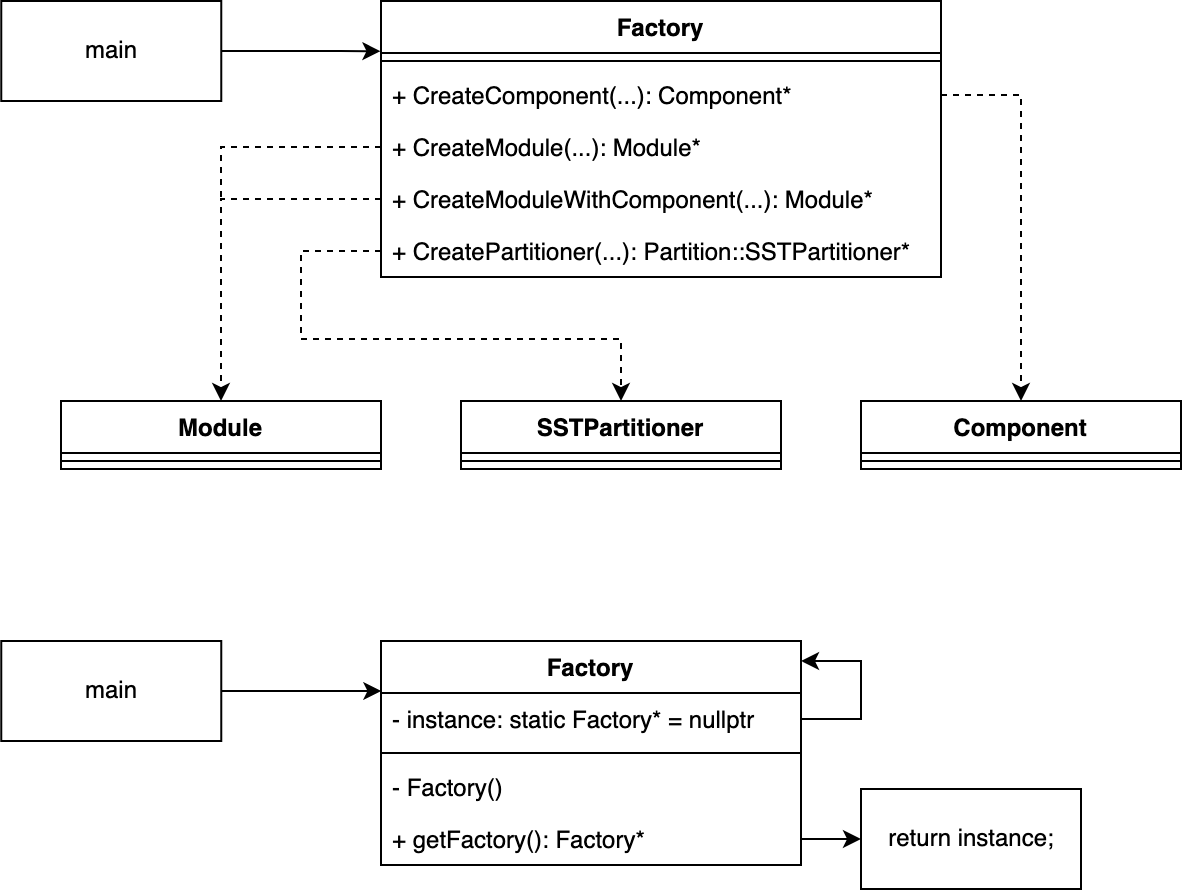
\includegraphics[width=0.8\textwidth]{af.png}
\end{figure}

Each of the methods accept parameters to instantiate the corresponding ConcreteProducts. There are several Client classes that call these methods, including \texttt{Simulation}, \texttt{BaseComponent} and the \texttt{main} function itself.



\subsection{Singleton Pattern}
The singleton pattern is present in the \texttt{Factory} and \texttt{Simulation.Simulation\_impl} classes. In the repository, the classes can be located at \texttt{factory.h} and \texttt{Simulation\_impl.h} respectively.

\subsubsection{Factory}
The \texttt{Factory} class is used to instantiate other concrete simulation classes. SST requires objects to be synchronized throughout the kernel, especially since they can be running on a distributed system where race conditions can become major issues. The software forces these simulation objects to be Singletons.

\begin{figure}[ht]
  \caption{Factory Implementing the Singleton Pattern}
  \centering
  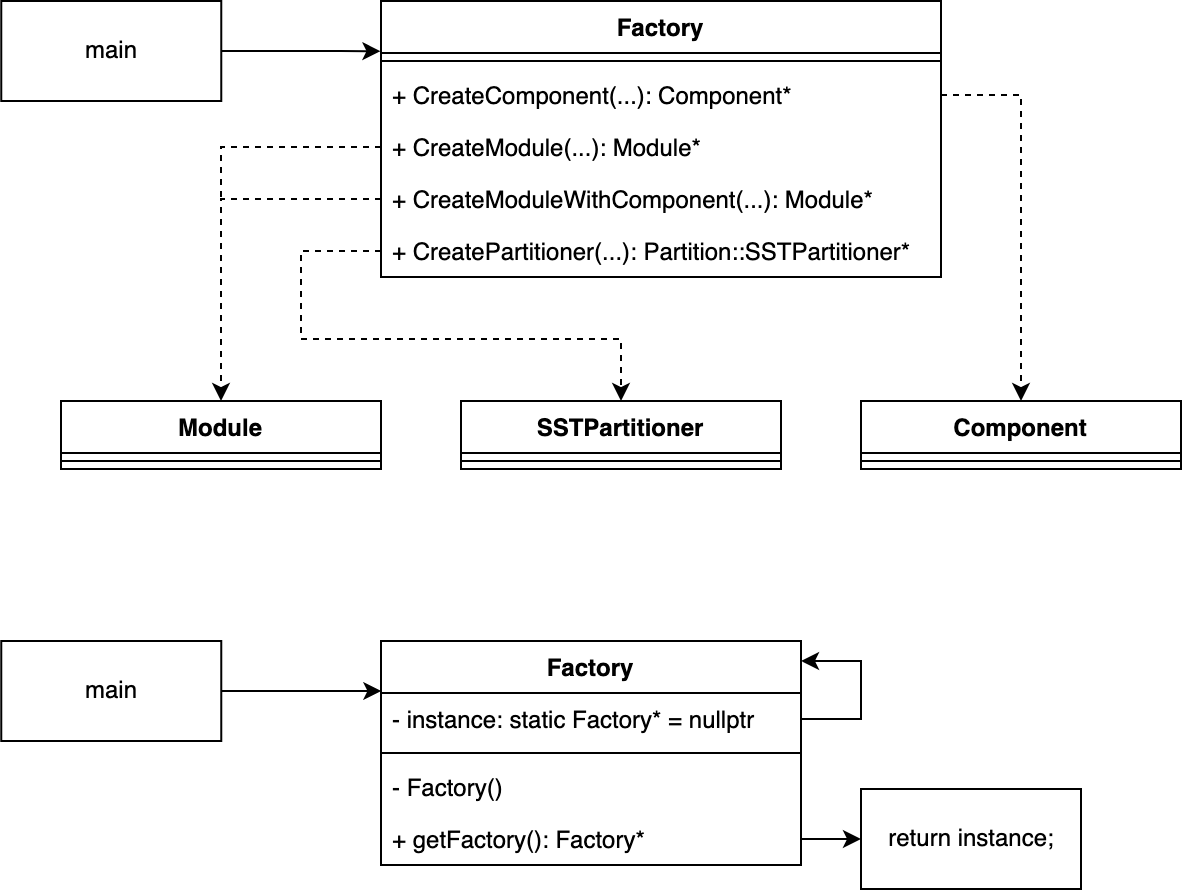
\includegraphics[width=0.8\textwidth]{singleton.png}
\end{figure}
\newpage

Listing \ref{singleton} demonstrates the \texttt{Factory} class following the typical steps dictated by the pattern.

\begin{lstlisting}[style=customC++,label=singleton,caption=Factory Implementing the Singleton Pattern \\ Files: src/sst/core/factory.h and src/sst/core/factory.cc]
class Factory {
  Factory(...);
  ~Factory();
  static Factory* instance;
}

Factory* Factory::instance = nullptr;

Factory::Factory(...) {
  if (instance) {
    ...
    // exit 1
  }
  instance = this;
}
\end{lstlisting}

Although SST is primarily intended for multi-threaded applications, the \texttt{Factory} Singleton class does not utilize any locks to account for the potential issues imposed by concurrency. Locks do exist in abundance throughout the project and within the class itself, but not when checking for instances of the class in other threads. The \texttt{Factory} class is responsible for creating SST Components, SubComponents, Modules, etc. as models for the simulation.

It appears that the Singleton is instantiated by \texttt{mpirun} as a single thread which spawns the other processes after it completes the analysis of the configuration options. The intent of the pattern is still preserved, although with the aforementioned assumptions that the executable instantiates it with a single thread.
\newpage

\subsubsection{Simulation\_impl}

\begin{figure}[ht]
  \caption{Simulation\_impl Implementing the Singleton Pattern}
  \centering
  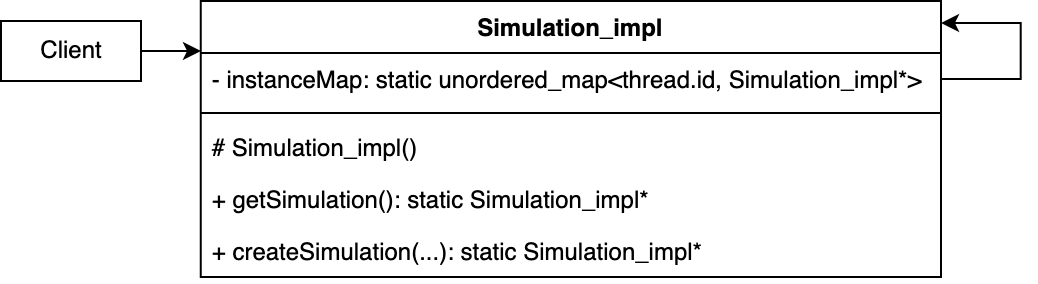
\includegraphics[width=0.8\textwidth]{singleton2.png}
\end{figure}

Listing \ref{simClassDecl} demonstrates the declaration of the other Singleton class, \texttt{Simulation\_impl}.

\begin{lstlisting}[style=customC++,label=simClassDecl,caption=Excerpt of Simulation\_impl Interface \\ File: src/sst/core/simulation\_impl.h]
class Simulation_impl : public Simulation {
public:
  static Simulation_impl* getSimulation();
  static Simulation_impl* createSimulation();
  static void shutdown();
protected:
  Simulation_impl(...) {}
private:
  static std::unordered_map<std::thread::id, Simulation_impl*> instanceMap;
}
\end{lstlisting}

Unlike \texttt{Factory}, this class is used by multiple classes in the framework which potentially may be on multiple threads. The \texttt{Simulation\_impl} class does implement a relatively safer version of a Singleton instance by using a mutex.

Listing \ref{singleton2} demonstrates the \texttt{Simulation\_impl} class following the typical steps dictated by the pattern, using a mutex to account for potential issues raised by multi-threaded processes.

\begin{lstlisting}[style=customC++,label=singleton2,caption=Simulation\_impl Implementing the Singleton Pattern \\ File: src/sst/core/simulation\_impl.cc]
std::unordered_map<std::thread::id, Simulation_impl*>
  Simulation_impl::instanceMap;

Simulation_impl* getSimulation() {
  return instanceMap.at(std::this_thread::get_id());
}

Simulation_Impl::createSimulation(...) {
  std::thread::id tid = std::this_thread::get_id();
  Simulation_impl* instance = new Simulation_impl(...);

  std::lock_guard<std::mutex> lock(simulationMutex);
  instanceMap[tid] = instance;
  ...
  return instance;
}

void Simulation_impl::shutdown() {
  instanceMap.clear();
}
\end{lstlisting}

\texttt{Simulation\_impl} appears to create an instance of itself on every thread and store them in the static unordered\_map attribute, instanceMap. Each of the instances follows the restrictions enacted by the Singleton pattern. This method allows for a Singleton object on every thread and therefore the core intent of the pattern remains preserved. The map's contents are destroyed with the public \texttt{shutdown} method which is accessible by the main function, which runs on the primary thread.


\subsection{Prototype Pattern}
The Prototype pattern is present in the project, although in a very limited manner. Select \texttt{SST::Core::Interfaces} classes implement a \texttt{clone} method to provide the ability to copy instances of themselves. The \texttt{StringEvent} class provides a shallow copy of itself to instantiate its ConcretePrototype, while \texttt{SimpleNetwork::Request} performs a deep copy.

\begin{figure}[h]
    \caption{Factory Implementing the Prototype Pattern}
    \centering
    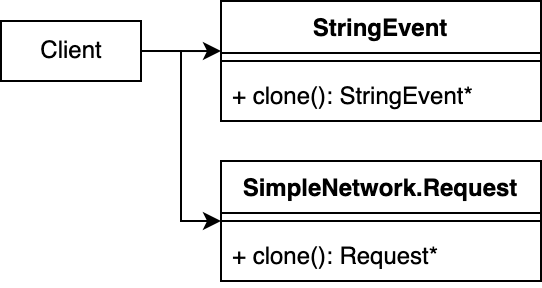
\includegraphics[width=0.8\textwidth]{proto.png}
\end{figure}

The following listings demonstrate the instances of the project following the typical steps dictated by the pattern:

\begin{lstlisting}[style=customC++,label=prototype1,caption=StringEvent Implementing the Prototype Pattern \\ File: src/sst/core/interfaces/stringEvent.h]
class StringEvent : public SST::Event, ... {
  virtual Event* clone() override {
    return new StringEvent(*this);
  }
}
\end{lstlisting}

\begin{lstlisting}[style=customC++,label=prototype2,caption=SimpleNetwork::Request Implementing the Prototype Pattern \\ File: src/sst/core/interfaces/simpleNetwork.h]
class SimpleNetwork : public SubComponent {
  class Request : public ... {
    Request* clone() {
      Request* req = new Request(*this);
      if (payload != nullptr) {
        req->payload = payload->clone();
      }
      return req;
    }
  }
}
\end{lstlisting}
